\documentclass[a4paper,twoside]{article}

\usepackage{epsfig}
\usepackage{graphicx} 
\usepackage{subcaption}
\usepackage{calc}
\usepackage{amssymb}
\usepackage{amstext}
\usepackage{amsmath}
\usepackage{amsthm}
\usepackage{multicol}
\usepackage{pslatex}
\usepackage{apalike}
\usepackage{algorithm2e}
\usepackage[bottom]{footmisc}
\usepackage{SCITEPRESS}     % Please add other packages that you may need BEFORE the SCITEPRESS.sty package.
\usepackage{siunitx}
\usepackage{booktabs}
\usepackage{threeparttable}
\usepackage{adjustbox}
\usepackage{multirow}
\usepackage{colortbl}
\usepackage{algorithmic}

\definecolor{gray!20}{rgb}{0.8,0.8,0.8}

\begin{document}

\title{Solving the Capacitated Vehicle Routing Problem \\with Graph Transformers}

\author{\authorname{Evgeny Polyachenko\sup{1}\orcidAuthor{0000-0002-4596-1222}, Daniel Antunes Pedrozo\sup{1}\orcidAuthor{0009-0005-0718-3908}, Jorge Augusto Meira\sup{1}\orcidAuthor{0000-0002-4086-5784}, and Radu State\sup{1}\orcidAuthor{0000-0002-4751-9577}}
\affiliation{\sup{1}2Interdisciplinary Centre for Security, Reliability and Trust, University of Luxembourg, Luxembourg}
\email{\{evgeny.polyachenko, jorge.meria\}@uni.lu}
}

\keywords{Vehicle Routing Problem, Graph Attention Network, Reinforcement Learning}

\abstract{This paper presents a novel approach to solving the Capacitated Vehicle Routing Problem (CVRP) using Graph Transformers. We leverage the power of deep reinforcement learning to train an agent that can dynamically construct high-quality routes for a fleet of vehicles. Our model is evaluated on a set of well-known CVRP benchmarks, and we show that it outperforms existing methods in terms of both solution quality and computational time.}




\onecolumn \maketitle \normalsize \setcounter{footnote}{0} \vfill

\section{\uppercase{Introduction}}
\label{sec:introduction}

\section{Model settings}

The Capacitated Vehicle Routing Problem (CVRP) studied in our benchmark consists of finding minimum-cost routes for a fleet of homogeneous vehicles to service a set of customers with known demands. Each vehicle has a fixed capacity, starts and ends its route at a central depot, and each customer must be visited exactly once by exactly one vehicle.

\subsection{Instance Generation}

CVRP instances are generated with the following specifications:

\begin{itemize}
    \item \textbf{Number of customers}: $n \in \{7, 8, 9, 10, \ldots, 20\}$ (varies by experiment)
    \item \textbf{Depot location}: Node $0$ with coordinates sampled uniformly
    \item \textbf{Customer locations}: Nodes $1, 2, \ldots, n$ with coordinates sampled uniformly
    \item \textbf{Coordinate generation}: 
        \begin{enumerate}
            \item Sample integer coordinates $(x_i, y_i) \sim \text{Uniform}\{0, 1, \ldots, 100\}$ for all nodes $i \in \{0, 1, \ldots, n\}$
            \item Normalize to unit square: $(x_i', y_i') = (x_i/100, y_i/100)$
        \end{enumerate}
    \item \textbf{Customer demands}: $q_i \sim \text{Uniform}\{1, 2, \ldots, 10\}$ for $i \in \{1, \ldots, n\}$
    \item \textbf{Depot demand}: $q_0 = 0$
    \item \textbf{Vehicle capacity}: $Q = 30$ (fixed for all instances)
    \item \textbf{Distance metric}: Euclidean distance in the normalized unit square
    %\item \textbf{Random seed}: $\text{seed} = 4242 + n \times 1000 + \text{instance\_id} \times 10 + \text{attempt}$
	\item \textbf{Random seed}: $\text{seed} = 1000 * n + i$ (where $i$ is instance id$- 1$)
\end{itemize}

\subsection{Mathematical Formulation}

Let $\mathcal{V} = \{0, 1, \ldots, n\}$ denote the set of all nodes, where node $0$ represents the depot and $\mathcal{N} = \{1, 2, \ldots, n\}$ represents the set of customers. Let $\mathcal{K}$ denote the set of available vehicles (unbounded in our formulation).

\subsubsection{Parameters}
\begin{itemize}
    \item $(x_i, y_i) \in [0, 1]^2$: Normalized coordinates of node $i \in \mathcal{V}$
    \item $d_{ij} = \sqrt{(x_i - x_j)^2 + (y_i - y_j)^2}$: Euclidean distance between nodes $i$ and $j$
    \item $q_i \in \{1, 2, \ldots, 10\}$: Demand of customer $i \in \mathcal{N}$ (with $q_0 = 0$)
    \item $Q = 30$: Vehicle capacity
\end{itemize}

\subsubsection{Decision Variables}
\begin{itemize}
    \item $x_{ijk} \in \{0, 1\}$: Binary variable equal to 1 if vehicle $k$ travels directly from node $i$ to node $j$
    \item $u_i \in [0, Q]$: Cumulative demand served when visiting node $i$ (for subtour elimination)
\end{itemize}

\subsubsection{Objective Function}
Minimize the total travel distance:
\begin{equation}
\min \sum_{k \in \mathcal{K}} \sum_{i \in \mathcal{V}} \sum_{j \in \mathcal{V}} d_{ij} \cdot x_{ijk}
\end{equation}

\subsubsection{Constraints}

\textbf{1. Each customer is visited exactly once:}
\begin{equation}
\sum_{k \in \mathcal{K}} \sum_{i \in \mathcal{V}, i \neq j} x_{ijk} = 1 \quad \forall j \in \mathcal{N}
\end{equation}

\textbf{2. Flow conservation (route continuity):}
\begin{equation}
\sum_{i \in \mathcal{V}, i \neq h} x_{ihk} = \sum_{j \in \mathcal{V}, j \neq h} x_{hjk} \quad \forall h \in \mathcal{V}, \forall k \in \mathcal{K}
\end{equation}

\textbf{3. Each vehicle starts from the depot:}
\begin{equation}
\sum_{j \in \mathcal{N}} x_{0jk} \leq 1 \quad \forall k \in \mathcal{K}
\end{equation}

\textbf{4. Each vehicle returns to the depot:}
\begin{equation}
\sum_{i \in \mathcal{N}} x_{i0k} \leq 1 \quad \forall k \in \mathcal{K}
\end{equation}

\textbf{5. Vehicle capacity constraint:}
\begin{equation}
\sum_{i \in \mathcal{N}} \sum_{j \in \mathcal{V}, j \neq i} q_i \cdot x_{ijk} \leq Q \quad \forall k \in \mathcal{K}
\end{equation}

\textbf{6. Subtour elimination (Miller-Tucker-Zemlin):}
\begin{equation}
u_i - u_j + Q \cdot x_{ijk} \leq Q - q_j \quad \forall i, j \in \mathcal{N}, i \neq j, \forall k \in \mathcal{K}
\end{equation}
\begin{equation}
q_i \leq u_i \leq Q \quad \forall i \in \mathcal{N}
\end{equation}

\subsection{Solution Representation}

A CVRP solution is represented as a set of vehicle routes, where each route is a sequence of customer nodes. The solution format used in the implementation is:

\begin{itemize}
    \item \textbf{Individual routes}: Each vehicle route is stored as a list $[c_1, c_2, \ldots, c_m]$ containing only customer nodes
    \item \textbf{Complete solution}: A list of vehicle routes $\mathcal{R} = \{r_1, r_2, \ldots, r_{|\mathcal{K}|}\}$
    \item \textbf{Flattened representation}: For output, routes are combined with explicit depot nodes: $[0, c_{11}, \ldots, c_{1m_1}, 0, c_{21}, \ldots, c_{2m_2}, 0, \ldots]$
\end{itemize}

\subsection{Solution Validation Procedure}

The following algorithm validates a CVRP solution and computes its objective value:

\begin{algorithm}
\caption{CVRP Solution Validation}
\begin{algorithmic}[1]
\REQUIRE Solution $\mathcal{R} = \{r_1, r_2, \ldots, r_K\}$, instance data $(d_{ij}, q_i, Q)$
\ENSURE Feasibility status and total cost

\STATE $\text{visited} \leftarrow \emptyset$ \COMMENT{Track visited customers}
\STATE $\text{total\_cost} \leftarrow 0$
\STATE $\text{feasible} \leftarrow \text{true}$

\FOR{each route $r_k \in \mathcal{R}$}
    \STATE $\text{route\_demand} \leftarrow 0$
    \STATE $\text{route\_cost} \leftarrow d_{0, r_k[1]}$ \COMMENT{Depot to first customer}
    
    \FOR{$i = 1$ to $|r_k|$}
        \IF{$r_k[i] \in \text{visited}$}
            \STATE $\text{feasible} \leftarrow \text{false}$ \COMMENT{Customer visited twice}
            \RETURN $(\text{false}, \infty)$
        \ENDIF
        \STATE $\text{visited} \leftarrow \text{visited} \cup \{r_k[i]\}$
        \STATE $\text{route\_demand} \leftarrow \text{route\_demand} + q_{r_k[i]}$
        
        \IF{$i < |r_k|$}
            \STATE $\text{route\_cost} \leftarrow \text{route\_cost} + d_{r_k[i], r_k[i+1]}$
        \ELSE
            \STATE $\text{route\_cost} \leftarrow \text{route\_cost} + d_{r_k[i], 0}$ \COMMENT{Last customer to depot}
        \ENDIF
    \ENDFOR
    
    \IF{$\text{route\_demand} > Q$}
        \STATE $\text{feasible} \leftarrow \text{false}$ \COMMENT{Capacity violated}
        \RETURN $(\text{false}, \infty)$
    \ENDIF
    
    \STATE $\text{total\_cost} \leftarrow \text{total\_cost} + \text{route\_cost}$
\ENDFOR

\IF{$|\text{visited}| \neq n$}
    \STATE $\text{feasible} \leftarrow \text{false}$ \COMMENT{Not all customers visited}
    \RETURN $(\text{false}, \infty)$
\ENDIF

\RETURN $(\text{true}, \text{total\_cost})$
\end{algorithmic}
\end{algorithm}

\subsection{Distance Calculation}

The exact Euclidean distance calculation used in the implementation:

\begin{algorithm}
\caption{Distance Matrix Computation}
\begin{algorithmic}[1]
\REQUIRE Coordinates $\{(x_i, y_i)\}_{i=0}^n$
\ENSURE Distance matrix $D \in \mathbb{R}^{(n+1) \times (n+1)}$

\FOR{$i = 0$ to $n$}
    \FOR{$j = 0$ to $n$}
        \STATE $D[i][j] \leftarrow \sqrt{(x_i - x_j)^2 + (y_i - y_j)^2}$
    \ENDFOR
\ENDFOR
\RETURN $D$
\end{algorithmic}
\end{algorithm}

\subsection{Instance Generation Algorithm}

The complete instance generation procedure as implemented:

\begin{algorithm}
\caption{CVRP Instance Generation}
\begin{algorithmic}[1]
\REQUIRE Number of customers $n$, instance ID $id$, attempt number $a$
\ENSURE CVRP instance $(coords, demands, distances, capacity)$
% \STATE $\text{seed} \leftarrow 4242 + n \times 1000 + id \times 10 + a$
\STATE $\text{seed} \leftarrow 1000 * n + i$

% $\text{seed} = 1000 * n + i$ (where $i$ is instance_id$- 1)

\STATE Set random seed to $\text{seed}$

\STATE \textbf{// Generate coordinates}
\FOR{$i = 0$ to $n$}
    \STATE $x_i \leftarrow \text{RandomInt}(0, 100)$
    \STATE $y_i \leftarrow \text{RandomInt}(0, 100)$
    \STATE $\text{coords}[i] \leftarrow (x_i/100, y_i/100)$
\ENDFOR

\STATE \textbf{// Generate demands}
\STATE $\text{demands}[0] \leftarrow 0$ \COMMENT{Depot has no demand}
\FOR{$i = 1$ to $n$}
    \STATE $\text{demands}[i] \leftarrow \text{RandomInt}(1, 10)$
\ENDFOR

\STATE \textbf{// Compute distance matrix}
\STATE $\text{distances} \leftarrow \text{ComputeDistanceMatrix}(\text{coords})$

\STATE \textbf{// Set capacity}
\STATE $\text{capacity} \leftarrow 30$

\RETURN $(\text{coords}, \text{demands}, \text{distances}, \text{capacity})$
\end{algorithmic}
\end{algorithm}

\subsection{Key Implementation Notes}

\begin{enumerate}
    \item \textbf{Coordinate Precision}: Coordinates are first sampled as integers from $\{0, 1, \ldots, 100\}$ then normalized to $[0, 1]$ by dividing by 100, ensuring consistent precision across instances.
    
    \item \textbf{Distance Computation}: Distances are computed using double-precision floating-point arithmetic to minimize rounding errors.
    
    \item \textbf{Vehicle Fleet}: The number of vehicles is unbounded (sufficient vehicles are always available), making this effectively a fleet-size-and-mix VRP with homogeneous unlimited vehicles.
    
    \item \textbf{Solution Quality}: Solutions are evaluated solely by total distance traveled; the number of vehicles used is not part of the objective function.
    
    \item \textbf{Reproducibility}: The deterministic seeding scheme ensures that instances can be exactly reproduced given the problem size, instance ID, and attempt number.
\end{enumerate}

% Embed this block inside Section "Model settings" (e.g., after the formulation)

\subsection{Key differences vs. Daniel's thesis that can worsen the optimal solution.}
\begin{itemize}
    \item \textbf{Forced use of every vehicle (Daniel's thesis) vs. optional use (this paper).}
    Daniel's thesis imposes per-vehicle equalities at the depot (each vehicle must depart and return exactly once), which \emph{forces all $|M|$ vehicles to be used}. If $|M|$ exceeds what is actually needed to minimize distance, this restriction can strictly \emph{increase} the optimal travel cost by splitting demand across unnecessary routes. In this paper, the depot constraints are inequalities ($\leq 1$), allowing unused vehicles and thus never forcing extra tours.
    
    \item \textbf{Fixed fleet size (Daniel's thesis) vs. unbounded fleet here.}
    Combined with the previous point, a fixed fleet that \emph{must} all be used can degrade the optimum when the fleet is larger than necessary for the instance, again increasing the total traveled distance. (By contrast, the unbounded-fleet model in this paper cannot worsen the distance-only objective, because it never forces the use of extra vehicles.)
    
    \item \textbf{MTZ subtour elimination here vs. load-flow formulation in Daniel's thesis (practical optimality under time limits).}
    While both are exact if solved to proven optimality, the MTZ (big-$M$) formulation used here typically has a \emph{weaker LP relaxation} than the single-commodity load-flow model in Daniel's thesis. Under realistic solver time limits or heuristic search, this weaker relaxation can lead to \emph{worse incumbent (higher-cost) solutions} being returned before optimality is proven.
\end{itemize}

\paragraph{Why the MTZ (big-$M$) model here can return worse solutions under time limits (novice explanation).}
\begin{itemize}
  \item \textbf{How MILP solvers search.} Solvers (Branch-and-Bound) repeatedly solve a relaxed version of the model where binary decisions are allowed to be fractional (between 0 and 1). This is called the \emph{LP relaxation}. Two things matter in practice:
  \begin{enumerate}
    \item a \emph{lower bound} from the relaxation (an optimistic cost that no true integer solution can beat), and
    \item the current best \emph{incumbent} (a feasible integer solution).
  \end{enumerate}
  Tighter relaxations give better (less optimistic) lower bounds and usually shrink the search effort, helping the solver find better incumbents within a fixed time.

  \item \textbf{What “weaker” means here.} In the MTZ model used in this paper, subtours are blocked with big-$M$ inequalities involving the $u_i$ variables (e.g., $u_i - u_j + Q\,x_{ijk} \le Q - q_j$). When $x_{ijk}$ is fractional in the relaxation (say $0.3$ or $0.5$), it is often easy to choose $u$ values so that these inequalities still hold. Intuitively, the relaxation can “pretend” that a fraction of a vehicle partially visits many customers at once. This produces LP solutions that look artificially cheap and very different from any real set of routes, i.e., the lower bound is \emph{too optimistic}. The solver then must branch a lot to repair these fractions, which consumes time and can delay finding high-quality incumbents.

  \item \textbf{Why Daniel’s thesis (load-flow) is stronger.} In Daniel’s thesis, every used arc must carry a consistent amount of \emph{load} $\ell_{ijm}$:
  \begin{itemize}
    \item If an arc $(i,j)$ is used (even fractionally in the relaxation), the load on it must be at least the demand of the next customer ($q_j\,x_{ijm} \le \ell_{ijm}$) and at most the remaining capacity.
    \item Load is \emph{conserved}: total load flowing into a customer minus the load flowing out must equal that customer’s demand.
  \end{itemize}
  These flow and capacity couplings make it much harder for the relaxation to “cheat” with fractional vehicles visiting many customers simultaneously. As a result, the LP relaxation is \emph{closer to the true integer problem} (a “stronger” relaxation), giving tighter lower bounds and guiding the search more effectively.

  \item \textbf{Practical outcome under time limits.} If you stop the solver early (as is common for larger CVRP instances), a weaker relaxation (MTZ) tends to:
  \begin{itemize}
    \item explore larger search trees (more time spent fixing fractional artifacts),
    \item provide looser bounds (less guidance),
    \item and, consequently, return \emph{worse incumbents} (higher cost routes) on average within the same time budget.
  \end{itemize}
  A stronger relaxation (load-flow from Daniel’s thesis) typically does the opposite: smaller trees, tighter bounds, and better incumbents sooner.

  \item \textbf{Important caveat.} If the solver runs to \emph{proven optimality}, both formulations reach the same optimum. The difference matters most when time or memory limits prevent full optimality proofs.
\end{itemize}



\subsection{GAT}


\subsection{GT}


\section{Optimal and suboptimal benchmarks}

\begin{figure*}[t!]
\centering
   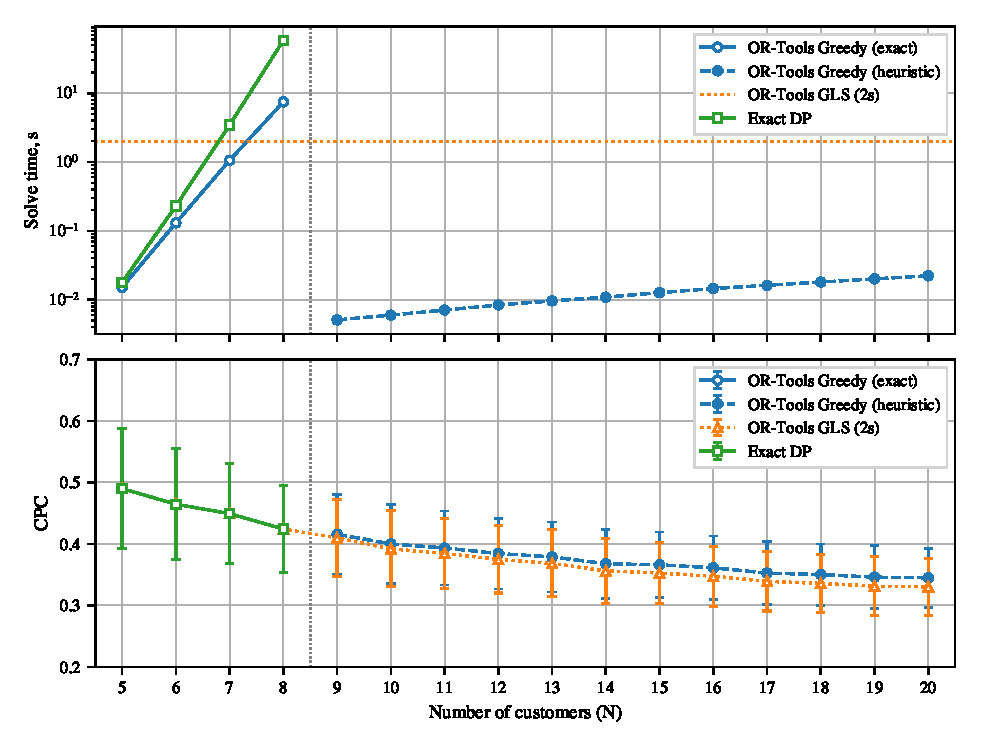
\includegraphics[width=160mm]{figures/benchmark.eps}
   \caption{Performance comparison of CVRP solvers on CPU benchmarks. 
       \textbf{Top panel:} Solve time (log scale) versus problem size for different solvers. 
       Exact DP provides optimal solutions but is limited to small instances (N$\leq$8). 
       OR-Tools Greedy operates in exact mode for N$\leq$8 (solid line) and switches to heuristic mode for larger instances (dashed line). 
       OR-Tools GLS with 2-second time limit maintains consistent performance across all problem sizes (dotted line). 
       \textbf{Bottom panel:} Cost per customer (CPC) showing solution quality with error bars indicating standard deviation across 1000 instances per problem size. 
       The vertical line at N=8.5 marks the transition point between exact and heuristic approaches for OR-Tools Greedy.}
\label{fig:benchmark}
% trim={5pt 10pt 5pt 8pt}, clip
\end{figure*}

\begin{figure}[t!]
\centering
   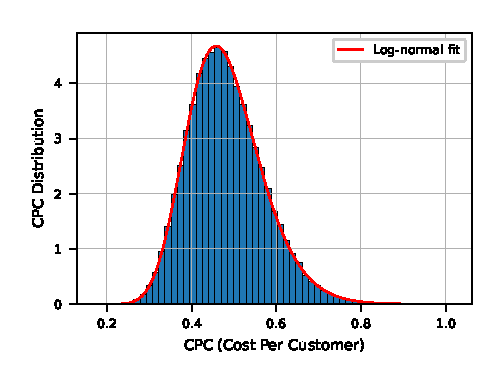
\includegraphics[width=80mm]{figures/cpc_histogram_paper_100k.eps}
   \caption{Distribution of CPC for N=10 CVRP instances solved using GPU dynamic programming. The histogram shows 100,000 random instances with the fitted log-normal distribution overlaid ($\mu=-0.748$, $\sigma=0.183$). The log-normal fit demonstrates that CPC follows a log-normal distribution (Kolmogorov-Smirnov test, $p=0.189$).}
\label{fig:cpc_histogram}
% trim={5pt 10pt 5pt 8pt}, clip
\end{figure}


\begin{figure}[t!]
\centering
   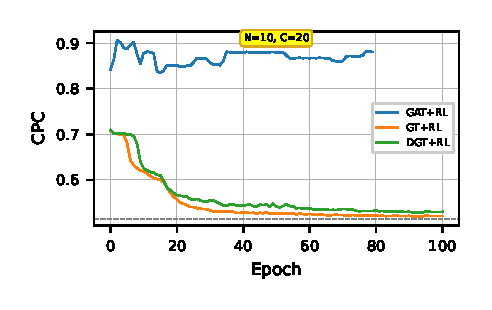
\includegraphics[width=80mm]{figures/tiny_n10.eps}
   \caption{Training batch 75}
\label{fig:training_batch}
% trim={5pt 10pt 5pt 8pt}, clip
\end{figure}



\begin{table*}[htbp]
\centering
\caption{Cost per Customer (CPC) for various CVRP sizes}
\label{tab:benchmark-comparison}
\small
\begin{tabular}{@{}l c c r r r r c c c c@{}}
\toprule
\textbf{Method} & \textbf{N} & \textbf{Cap.} & \textbf{Time} & \textbf{Mean} & \textbf{GM} & \textbf{Median} & \textbf{Error} & \textbf{95\% Range} & \textbf{KS CPC} & \textbf{KS log(CPC)} \\
\midrule
GPU-DP-Exact (sub)   & 8  & 30 & -- & 0.4265 & 0.4206 & 0.4237 & 9.07e-05 & [0.2966, 0.5696] & $<0.01$ & $<0.01$ \\
CPU-DP-Exact (opt)    & 8 & 30 & 58.54s & 0.4241 & 0.4182 & 0.4213 & 3.01e-03 & [0.2957, 0.5653] & $0.46$ & $0.38$ \\
OR-Tools Greedy (opt) & 8 & 30 & 7.48s & 0.4241 & 0.4182 & 0.4213 & 3.01e-03 & [0.2957, 0.5653] & $0.46$ & $0.38$ \\
OR-Tools GLS (sub)    & 8 & 30 & 2.00s & 0.4241 & 0.4182 & 0.4213 & 3.01e-03 & [0.2957, 0.5653] & $0.46$ & $0.38$ \\
\midrule
% GPU-DP-Exact (opt?)   & 10 & 20 & -- & 0.4821 & 0.4740 & 0.4742 & 1.10e-04 & [0.3308, 0.6767] & $<0.01$ & $<0.01$ \\
% \midrule
GPU-DP-Exact (sub)   & 10 & 30 & --     & 0.3947 & 0.3900 & 0.3913 & 7.35e-05 & [0.2854, 0.5272] & $<0.01$ & $<0.01$ \\
OR-Tools GLS (sub)    & 10 & 30 & 2.00s  & 0.3920 & 0.3873 & 0.3884 & 2.39e-03 & [0.2858, 0.5259] & $0.13$ & $0.70$ \\
OR-Tools Greedy (sub) & 10 & 30 & 5.99ms & 0.4000 & 0.3950 & 0.3958 & 2.55e-03 & [0.2879, 0.5362] & $0.17$ & $0.97$ \\
\rowcolor{gray!20}  Paper I (SCIP opt)    & 10 & 30 & 6.7ms  & 0.4360 & -      & -      & -        & - & - &- \\             
\midrule
OR-Tools GLS (sub)    & 20 & 30 & 2.00s & 0.3301 & 0.3270 & 0.3284 & 1.93e-03 & [0.2469, 0.4261] & $0.20$ & $0.87$ \\
OR-Tools Greedy (sub) & 20 & 30 & 0.022s & 0.3448 & 0.3414 & 0.3439 & 1.88e-03 & [0.2547, 0.4461] & $0.68$ & $0.07$ \\
\rowcolor{gray!20}  Paper I (GR sub)      & 10 & 30 & 42ms  & 0.3550 & -      & -      & -        & - & - &- \\             
\bottomrule
\end{tabular}
\begin{tablenotes}
\small
\item - Statistics computed over $10^6/10^3$ instances for GPU-DP-Exact/Others per configuration
\item - CPU DP-Exact solver uses brute-force enumeration of all customer partitions and route permutations (${\cal O}(n! \times 2^n)$), ensuring truly optimal solutions but restricting feasibility to $N\le 8$.
\item - GPU ``DP-Exact'' solver combines optimal Held-Karp dynamic programming for partitioning (${\cal O}(n^2 2^n)$) with nearest neighbor heuristic for route ordering, achieving near-optimal solutions with dramatically improved scalability through GPU parallelization.
\item - Time: Average time required to solve 1 instance
\item - Mean: Arithmetic mean; GM: Geometric mean
\item - Error: Maximum of SE(Mean), SE(GM), SE(Median) where:
\item \quad SE(Mean) = $s/\sqrt{n}$; SE(GM) = $\text{GM} \times \log(\text{GSD})/\sqrt{n}$; SE(Median) via KDE
\item - 95\% Range: [2.5th percentile, 97.5th percentile] of CPC values
\item - KS: Kolmogorov-Smirnov test p-values for normality, CPC and log(CPC)
\item - (opt): optimal solver; (sub): sub-optimal solver
\item - Paper I: Pedrozo D.A. Integrating Machine Learning and Optimisation to ...
\end{tablenotes}
\end{table*}


\begin{table}[htbp]
\centering
\caption{Timing Comparison: Exact DP vs OR-Tools Greedy (Optimal Mode)}
\label{tab:timing-comparison}
\small
\begin{tabular}{@{}c c c c c c c@{}}
\toprule
\textbf{N} & \textbf{Exact DP} & \textbf{OR-Tools} & \textbf{1K Exact} & \textbf{1K OR-Tools} & \textbf{10K Exact} & \textbf{10K OR-Tools} \\
\midrule
5 & 18ms & 15ms & 0.3m & 0.2m & 3.0m & 2.5m \\
6 & 230ms & 131ms & 3.8m & 2.2m & 38.3m & 21.8m \\
7 & 3.5s & 1.1s & 57.5m & 17.7m & 09.35h & 02.56h \\
8 & 58.5s & 7.5s & 16.15h & 02.04h & 06.18d & 20.46h \\
\midrule
9 & 19.3m & 48.2s & 13.08d & 13.22h & 133.17d & 05.13d \\
10 & 7.3h & 4.6m & 303.12d & 03.05d & 3035.09d & 32.04d \\
\bottomrule
\end{tabular}
\begin{tablenotes}
\small
\item Single instance timing per method (N=5-8: actual data; N=9-10: quadratic extrapolation)
\item 1K/10K columns show total time for 1,000/10,000 instances
\item Time format: ms=milliseconds, s=seconds, m=minutes, h=hours (HH.MM), d=days (DD.HH)
\item OR-Tools run in optimal mode with same solution quality as Exact DP
\end{tablenotes}
\end{table}


\begin{table*}[htbp] 
\centering
\caption{Optimal and sub-optimal (OR-Tools GLS) CPC values (10k instances per configuration)}
\label{tab:ortools-gls-timeout}
\small \begin{tabular}{@{}l c c c S[table-format=1.4] S[table-format=1.4] c c c c c c@{}}
\toprule
\textbf{Method} & \textbf{N} & \textbf{Cap.} & \textbf{Timeout} & {\textbf{GM}} & {\textbf{GSD}} & \textbf{95\% Range} & \textbf{95\% CI} & \textbf{KS} \\
\midrule
Exact DP (1000k). & 8 & 30 &-- & 0.4206 & 1.1833 & [0.3024, 0.5850] & [0.4204, 0.4207] & $<$0.01 \\
Exact DP (1000k)* & 8 & 30 &-- & 0.4237 & nan    & [0.2966, 0.5696] & [0.0003, 0.0006] & $<$0.01 \\
\midrule
Exact (100k) & 10 & 20 & -- & 0.4735 & 1.2012 & [0.3306, 0.6782] & [0.4730, 0.4741] & $0.19$  \\
Exact (10k)  & 10 & 20 & -- & 0.4737 & 1.1996 & [0.3316, 0.6767] & [0.4720, 0.4754] & $0.93$  \\
Heuristic    & 10 & 20 & 2s & 0.4744 & 1.2025 & [0.3305, 0.6809] & [0.4727, 0.4761] & $0.91$  \\
\midrule
Heuristic    & 20 & 30 & 2s & 0.3257 & 1.1473 & [0.2488, 0.4264] & [0.3248, 0.3266] & $0.15$  \\
Heuristic    & 20 & 30 & 10s & 0.3234 & 1.1459 & [0.2477, 0.4224] & [0.3226, 0.3243] & $0.08$ \\
\midrule
Heuristic    & 50 & 40 & 10s & 0.2366 & 1.1233 & [0.1884, 0.2972] & [0.2270, 0.2467] & $0.89$  \\
Heuristic    & 50 & 40 & 20s & 0.2391 & 1.1270 & [0.1892, 0.3023] & [0.2323, 0.2462] & $0.05$  \\
Heuristic    & 50 & 40 & 30s & 0.2253 & 1.1294 & [0.1775, 0.2860] & [0.2247, 0.2258] & $<0.01$ \\
Heuristic    & 50 & 40 & 60s & 0.2237 & 1.1293 & [0.1763, 0.2839] & [0.2232, 0.2243] & $<0.01$ \\
\midrule
Heuristic    & 100 & 50 & 10s & 0.1729 & 1.1061 & [0.1419, 0.2108] & [0.1676, 0.1784] & $<0.01$  \\
Heuristic    & 100 & 50 & 20s & 0.1673 & 1.1353 & [0.1305, 0.2146] & [0.1612, 0.1737] & $<0.01$  \\
Heuristic    & 100 & 50 & 30s & 0.1552 & 1.0338 & [0.1454, 0.1657] & [0.1538, 0.1567] & $<0.01$  \\
Heuristic    & 100 & 50 & 60s & 0.1754 & 1.1258 & [0.1391, 0.2213] & [0.1750, 0.1758] & $<0.01$  \\
Heuristic.   & 100 & 50 & 120s & 0.1737 & 1.1259 & [0.1377, 0.2192] & [0.1733, 0.1741]& $<0.01$  \\
OR-Tools GLS & 100 & 50 & 240s & 0.1721 & 1.1265 & [0.1362, 0.2173] & [0.1717, 0.1725] & $<$0.01 \\
\bottomrule
\end{tabular}
\begin{tablenotes}
\small
\item Exact: 
\item Heuristic: OR-Tools GLS
\item GM: Geometric Mean, GSD: Geometric Standard Deviation
\item 95\% Range: GM $\times$ [GSD$^{-1.96}$, GSD$^{+1.96}$]
\item KS: Kolmogorov-Smirnov, D'Agost.: D'Agostino, JB: Jarque-Bera (p-values for log(CPC) normality)
\item AD: Anderson-Darling test statistic (critical value at 5\% = 0.787; * indicates rejection)
\item Timeout column indicates per-instance time limit used by OR-Tools GLS
\item Test run with 20 instances per configuration
\end{tablenotes}
\end{table*}

\end{document}



\begin{table*}[htbp] 
\centering
\caption{Optimal and sub-optimal (OR-Tools GLS) CPC values (10k instances per configuration)}
\label{tab:ortools-gls-timeout}
\small \begin{tabular}{@{}l c c c S[table-format=1.4] S[table-format=1.4] c c c c c c@{}}
\toprule
\textbf{Method} & \textbf{N} & \textbf{Cap.} & \textbf{Timeout} & {\textbf{GM}} & {\textbf{GSD}} & \textbf{95\% Range} & \textbf{95\% CI} & \textbf{KS} & \textbf{D'Agost.} & \textbf{JB} & \textbf{AD} \\
\midrule
Exact DP (1000k). & 8 & 30 &-- & 0.4206 & 1.1833 & [0.3024, 0.5850] & [0.4204, 0.4207] & $<$0.01 & $<$0.01 & $<$0.01 & $834.920*$ \\
Exact DP (1000k)* & 8 & 30 &-- & 0.4237 & nan & [0.2966, 0.5696] & [0.0003, 0.0006] & $<$0.01 & $<$0.01 & $<$0.01 & $834.920*$ \\
\midrule
Exact (100k) & 10 & 20 & -- & 0.4735 & 1.2012 & [0.3306, 0.6782] & [0.4730, 0.4741] & $0.19$ & $<$0.001 & $<$0.001 & $1.405^*$ \\
Exact (10k)  & 10 & 20 & -- & 0.4737 & 1.1996 & [0.3316, 0.6767] & [0.4720, 0.4754] & $0.93$ & $0.37$ & $0.37$ & $0.295$ \\
Heuristic    & 10 & 20 & 2s & 0.4744 & 1.2025 & [0.3305, 0.6809] & [0.4727, 0.4761] & $0.91$ & $0.08$ & $0.08$ & $0.503$ \\
\midrule
Heuristic    & 20 & 30 & 2s & 0.3257 & 1.1473 & [0.2488, 0.4264] & [0.3248, 0.3266] & $0.15$ & $<0.01$ & $<0.01$ & $1.711*$ \\
Heuristic    & 20 & 30 & 10s & 0.3234 & 1.1459 & [0.2477, 0.4224] & [0.3226, 0.3243] & $0.08$ & $<0.01$ & $<0.01$ & $2.136*$ \\
\midrule
Heuristic    & 50 & 40 & 10s & 0.2366 & 1.1233 & [0.1884, 0.2972] & [0.2270, 0.2467] & $0.89$ & $0.33$ & $0.55$ & $0.411$ \\
Heuristic    & 50 & 40 & 20s & 0.2391 & 1.1270 & [0.1892, 0.3023] & [0.2323, 0.2462] & $0.05$ & $0.12$ & $0.32$ & $1.580*$ \\
Heuristic    & 50 & 40 & 30s & 0.2253 & 1.1294 & [0.1775, 0.2860] & [0.2247, 0.2258] & $<0.01$ & $<0.01$ & $<0.01$ & $8.207*$ \\
Heuristic    & 50 & 40 & 60s & 0.2237 & 1.1293 & [0.1763, 0.2839] & [0.2232, 0.2243] & $<0.01$ & $<0.01$ & $<0.01$ & $8.666*$ \\
\midrule
Heuristic    & 100 & 50 & 10s & 0.1729 & 1.1061 & [0.1419, 0.2108] & [0.1676, 0.1784] & $<0.01$ & $ 0.09$ & $0.11$ & $2.018*$ \\
Heuristic    & 100 & 50 & 20s & 0.1673 & 1.1353 & [0.1305, 0.2146] & [0.1612, 0.1737] & $<0.01$ & $<0.01$ & $<0.01$ & $4.906*$ \\
Heuristic    & 100 & 50 & 30s & 0.1552 & 1.0338 & [0.1454, 0.1657] & [0.1538, 0.1567] & $<0.01$ & $<0.01$ & $0.06$ & $4.285*$ \\
Heuristic    & 100 & 50 & 60s & 0.1754 & 1.1258 & [0.1391, 0.2213] & [0.1750, 0.1758] & $<0.01$ & $<0.01$ & $<0.01$ & $14.709*$ \\
Heuristic.   & 100 & 50 & 120s & 0.1737 & 1.1259 & [0.1377, 0.2192] & [0.1733, 0.1741]& $<0.01$ & $<0.01$ & $<0.01$ & $15.276*$ \\
OR-Tools GLS & 100 & 50 & 240s & 0.1721 & 1.1265 & [0.1362, 0.2173] & [0.1717, 0.1725] & $<$0.01 & $<$0.01 & $<$0.01 & $16.739*$ \\
\bottomrule
\end{tabular}
\begin{tablenotes}
\small
\item Exact: 
\item Heuristic: OR-Tools GLS
\item GM: Geometric Mean, GSD: Geometric Standard Deviation
\item 95\% Range: GM $\times$ [GSD$^{-1.96}$, GSD$^{+1.96}$]
\item KS: Kolmogorov-Smirnov, D'Agost.: D'Agostino, JB: Jarque-Bera (p-values for log(CPC) normality)
\item AD: Anderson-Darling test statistic (critical value at 5\% = 0.787; * indicates rejection)
\item Timeout column indicates per-instance time limit used by OR-Tools GLS
\item Test run with 20 instances per configuration
\end{tablenotes}
\end{table*}



\begin{table*}[htbp]
\centering
\caption{Comparison of Mean, Geometric Mean, and Median with Standard Errors}
\label{tab:central-tendency-comparison}
\small
\begin{tabular}{@{}l c c c r r r c c c c@{}}
\toprule
\textbf{Method} & \textbf{N} & \textbf{Cap.} & \textbf{Timeout} & \textbf{Mean} & \textbf{GM} & \textbf{Median} & \textbf{Error} & \textbf{95\% Range} & \textbf{KS CPC} & \textbf{KS log(CPC)} \\
\midrule
GPU-DP-Exact & 8  & 30 & -- & 0.4265 & 0.4206 & 0.4237 & 9.07e-05 & [0.2966, 0.5696] & $<0.01$ & $<0.01$ \\
GPU-DP-Exact & 10 & 20 & -- & 0.4821 & 0.4740 & 0.4742 & 1.10e-04 & [0.3308, 0.6767] & $<0.01$ & $<0.01$ \\
GPU-DP-Exact & 10 & 30 & -- & 0.3947 & 0.3900 & 0.3913 & 7.35e-05 & [0.2854, 0.5272] & $<0.01$ & $<0.01$ \\
\bottomrule
\end{tabular}
\begin{tablenotes}
\small
\item Mean: Arithmetic mean; GM: Geometric mean
\item Error: Maximum of SE(Mean), SE(GM), SE(Median) where:
\item \quad SE(Mean) = $s/\sqrt{n}$; SE(GM) = $\text{GM} \times \log(\text{GSD})/\sqrt{n}$; SE(Median) via KDE at sample median
\item 95\% Range: [2.5th percentile, 97.5th percentile] of CPC values
\item KS: Kolmogorov-Smirnov test p-values for normality, CPC and log(CPC)
\end{tablenotes}
\end{table*}



\begin{table*}[htbp]
\centering
%\adjustbox{width=\textwidth}{%
\begin{tabular}{@{}l|ccccc@{}}
\toprule
\textbf{Parameter} & \textbf{Tiny} & \textbf{Small} & \textbf{Medium} & \textbf{Large} & \textbf{Huge} \\
\midrule
\multicolumn{6}{c}{\textbf{Problem Configuration}} \\
\midrule
Number of customers & 10 & 10 & 20 & 50 & 100 \\
Vehicle capacity & 20 & 20 & 30 & 40 & 50 \\
\midrule
\multicolumn{6}{c}{\textbf{Graph Transformer (GT/DGT) Architecture}} \\
\midrule
Hidden dimension & 128 & 128 & 256$^{\dagger}$ & 512 & 512 \\
Number of heads & 4$^{\dagger}$ & 4$^{\dagger}$ & 4$^{\dagger}$ & 8 & 8 \\
Number of layers & 3 & 3 & 4$^{\dagger}$ & 6 & 8 \\
Transformer dropout & 0.1$^{\dagger}$ & 0.1$^{\dagger}$ & 0.1$^{\dagger}$ & 0.15 & 0.2 \\
Feedforward multiplier & 2$^{\dagger}$ & 2$^{\dagger}$ & 2$^{\dagger}$ & 2$^{\dagger}$ & 2$^{\dagger}$ \\
\midrule
\multicolumn{6}{c}{\textbf{GAT Architecture}} \\
\midrule
GAT hidden dimension & 128 & 128 & 256$^{\dagger}$ & 512 & 512 \\
GAT layers & 3 & 3 & 4$^{\dagger}$ & 5 & 6 \\
GAT dropout & 0.6$^{\dagger}$ & 0.6$^{\dagger}$ & 0.6$^{\dagger}$ & 0.5 & 0.5 \\
GAT edge dimension & 16$^{\dagger}$ & 16$^{\dagger}$ & 16$^{\dagger}$ & 16$^{\dagger}$ & 16$^{\dagger}$ \\
GAT negative slope & 0.2$^{\dagger}$ & 0.2$^{\dagger}$ & 0.2$^{\dagger}$ & 0.2$^{\dagger}$ & 0.2$^{\dagger}$ \\
\midrule
\multicolumn{6}{c}{\textbf{Model Parameter Counts}} \\
\midrule
GAT total parameters & 320K & 320K & 1.28M & 6.83M & 10.2M \\
GT total parameters & 780K & 780K & 3.12M & 19.9M & 31.9M \\
DGT total parameters & 1.77M & 1.77M & 7.09M & 45.3M & 72.5M \\
\midrule
\multicolumn{6}{c}{\textbf{Training Configuration}} \\
\midrule
Batches per epoch$^{*}$ & 15 & 1500$^{\dagger}$ & 1500$^{\dagger}$ & 1500$^{\dagger}$ & 1500$^{\dagger}$ \\
Batch size & 64 & 512$^{\dagger}$ & 512$^{\dagger}$ & 512$^{\dagger}$ & 512$^{\dagger}$ \\
Number of epochs & 100$^{\dagger}$ & 100$^{\dagger}$ & 100$^{\dagger}$ & 100$^{\dagger}$ & 100$^{\dagger}$ \\
Learning rate & $10^{-4\dagger}$ & $10^{-4\dagger}$ & $10^{-4\dagger}$ & $10^{-4\dagger}$ & $10^{-4\dagger}$ \\
\midrule
\multicolumn{6}{c}{\textbf{Advanced Training (for Large/Huge)}} \\
\midrule
Early stopping patience & 10$^{\dagger}$ & 10$^{\dagger}$ & 10$^{\dagger}$ & 10$^{\dagger}$ & 40 \\
Gradient clip norm & 2.0$^{\dagger}$ & 2.0$^{\dagger}$ & 2.0$^{\dagger}$ & 2.0$^{\dagger}$ & 1.5 \\
\bottomrule
\end{tabular}%
% }
\caption{Configuration parameters for different problem scales in the Dynamic Graph Transformer RL framework. Values marked with $^{\dagger}$ represent default values from \texttt{default.yaml}. The tiny configuration uses reduced training data ($^{*}$batches per epoch = 15) for rapid experimentation, while other configurations use the full training regime. Model parameter counts are calculated based on the respective architectures: GAT (Graph Attention Network), GT (Graph Transformer), and DGT (Dynamic Graph Transformer).}
\label{tab:config_comparison}
\end{table*}


\begin{table*}[htbp]
\centering
\caption{OR-Tools Greedy Heuristic Performance (PATH\_CHEAPEST\_ARC Strategy)}
\label{tab:ortools-greedy}
\begin{tabular}{@{}c c c S[table-format=1.6] S[table-format=1.6] S[table-format=1.6] c@{}}
\toprule
\textbf{N} & \textbf{Capacity} & \textbf{Instances} & {\textbf{Mean CPC}} & {\textbf{Std CPC}} & {\textbf{SEM}} & \textbf{2×SEM/Mean(\%)} \\
\midrule
10  & 20 & 10 & 0.4557 & 0.0718 & 0.0227 & 9.97\% \\
20  & 30 & 10 & 0.3389 & 0.0398 & 0.0126 & 7.43\% \\
50  & 40 & 10 & 0.2515 & 0.0274 & 0.0087 & 6.90\% \\
100 & 50 & 10 & 0.1801 & 0.0188 & 0.0059 & 6.59\% \\
\bottomrule
\end{tabular}
\end{table*}

% Table 2: OR-Tools GLS (GUIDED_LOCAL_SEARCH)
\begin{table*}[htbp]
\centering
\caption{OR-Tools Guided Local Search Performance (GUIDED\_LOCAL\_SEARCH Metaheuristic)}
\label{tab:ortools-gls}
\begin{tabular}{@{}c c c S[table-format=1.6] S[table-format=1.6] S[table-format=1.6] c@{}}
\toprule
\textbf{N} & \textbf{Capacity} & \textbf{Instances} & {\textbf{Mean CPC}} & {\textbf{Std CPC}} & {\textbf{SEM}} & \textbf{2×SEM/Mean(\%)} \\
\midrule
10  & 20 & 10 & 0.4481 & 0.0708 & 0.0224 & 10.00\% \\
20  & 30 & 10 & 0.3245 & 0.0324 & 0.0102 & 6.32\% \\
50  & 40 & 10 & 0.2433 & 0.0276 & 0.0087 & 7.18\% \\
100 & 50 & 10 & 0.1776 & 0.0197 & 0.0062 & 7.02\% \\
\bottomrule
\end{tabular}
\end{table*}


10  & 20 & 0.4481 & 0.0708
20  & 30 & 0.3245 & 0.0324
50  & 40 & 0.2433 & 0.0276
100 & 50 & 0.1776 & 0.0197


\begin{table*}[htbp]
\centering
\caption{GPU Improved Heuristic Performance (100 instances)}
\label{tab:gpu-heuristic-100}
\begin{tabular}{@{}c c S[table-format=1.4] S[table-format=1.4] S[table-format=1.4] c@{}}
\toprule
\textbf{N} & \textbf{Capacity} & {\textbf{Mean CPC}} & {\textbf{Std CPC}} & {\textbf{SEM}} & \textbf{2×SEM/Mean(\%)} \\
\midrule
 10 & 20 & 0.4731 & 0.0834 & 0.0083 & 3.53\% \\ % exact-dp
 10 & 20 & 0.4845 & 0.0916 & 0.0092 & 3.78\% \\
 20 & 30 & 0.3367 & 0.0449 & 0.0045 & 2.67\% \\
 50 & 40 & 0.2317 & 0.0266 & 0.0027 & 2.30\% \\
100 & 50 & 0.1751 & 0.0169 & 0.0017 & 1.94\% \\
\bottomrule
\end{tabular}
\end{table*}


\begin{table*}[htbp]
\centering
\caption{GPU Improved Heuristic Performance (1,000 instances)}
\label{tab:gpu-heuristic-1000}
\begin{tabular}{@{}c c S[table-format=1.4] S[table-format=1.4] S[table-format=1.4] c@{}}
\toprule
\textbf{N} & \textbf{Capacity} & {\textbf{Mean CPC}} & {\textbf{Std CPC}} & {\textbf{SEM}} & \textbf{2×SEM/Mean(\%)} \\
\midrule
 10 & 20 & 0.4824 & 0.0904 & 0.0029 & 1.19\% \\ %exact-dp
 10 & 20 & 0.4932 & 0.0961 & 0.0030 & 1.23\% \\
 20 & 30 & 0.3388 & 0.0468 & 0.0015 & 0.87\% \\
 50 & 40 & 0.2312 & 0.0280 & 0.0009 & 0.77\% \\
100 & 50 & 0.1761 & 0.0205 & 0.0006 & 0.73\% \\
\bottomrule
\end{tabular}
\end{table*}



\begin{figure*}[t!]
\centering
   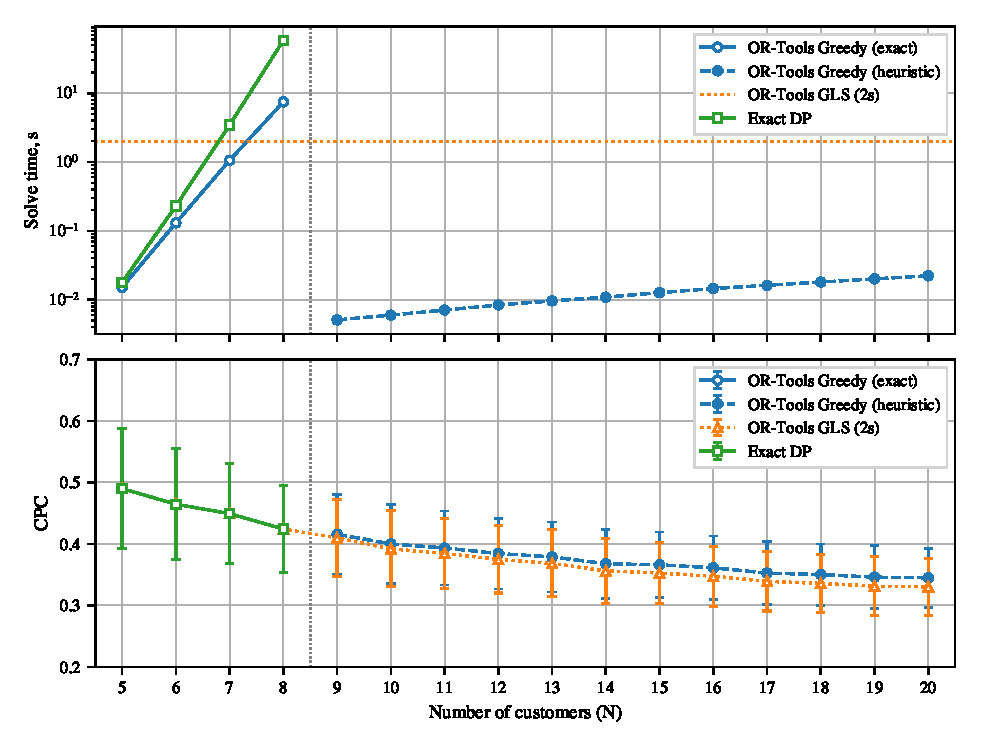
\includegraphics[width=160mm]{figures/benchmark.eps}
   \caption{Performance comparison of CVRP solvers on CPU benchmarks. 
       \textbf{Top panel:} Solve time (log scale) versus problem size for different solvers. 
       Exact DP provides optimal solutions but is limited to small instances (N$\leq$8). 
       OR-Tools Greedy operates in exact mode for N$\leq$8 (solid line) and switches to heuristic mode for larger instances (dashed line). 
       OR-Tools GLS with 2-second time limit maintains consistent performance across all problem sizes (dotted line). 
       \textbf{Bottom panel:} Cost per customer (CPC) showing solution quality with error bars indicating standard deviation across 1000 instances per problem size. 
       The vertical line at N=8.5 marks the transition point between exact and heuristic approaches for OR-Tools Greedy.}
\label{fig:benchmark_duplicate}
% trim={5pt 10pt 5pt 8pt}, clip
\end{figure*}

\begin{table*}[htbp]
\centering
\caption{GPU CVRP Performance with Log-normal Statistics and Normality Tests}
\label{tab:gpu-performance-complete}
\begin{tabular}{@{}l c c S[table-format=1.4] S[table-format=1.4] c c c c c c@{}}
\toprule
\textbf{Method} & \textbf{N} & \textbf{Cap.} & {\textbf{GM}} & {\textbf{GSD}} & 
\textbf{95\% Range} & \textbf{95\% CI} & \textbf{KS} & \textbf{D'Agost.} & \textbf{JB} & \textbf{AD} \\
\midrule
Exact (100k) & 10 & 20 & 0.4735 & 1.2012 & [0.3306, 0.6782] & [0.4730, 0.4741] & $0.19$ & $<$0.001 & $<$0.001 & $1.405^*$ \\
Exact (10k) & 10 & 20 & 0.4737 & 1.1996 & [0.3316, 0.6767] & [0.4720, 0.4754] & $0.93$ & $0.37$ & $0.37$ & $0.295$ \\
Heuristic & 10 & 20 & 0.4831 & 1.2064 & [0.3344, 0.6978] & [0.4813, 0.4849] & $0.87$ & $0.44$ & $0.44$ & $0.353$ \\
Heuristic* & 20 & 30 & 0.3319 & 1.1514 & [0.2518, 0.4376] & [0.3310, 0.3328] & $1.00$ & $0.85$ & $0.86$ & $0.093$ \\
Heuristic* & 50 & 40 & 0.2303 & 1.1291 & [0.1815, 0.2921] & [0.2297, 0.2308] & $0.73$ & $0.29$ & $0.28$ & $0.400$ \\
OR-Tools GLS & 100 & 50 & 0.1811 & 1.1058 & [0.1487, 0.2206] & [0.1776, 0.1847] & $0.47$ & $0.39$ & $0.49$ & $0.521$ \\
\bottomrule
\end{tabular}
\begin{tablenotes}
\small
\item GM: Geometric Mean, GSD: Geometric Standard Deviation
\item 95\% Range: Individual value range GM $\times$ [GSD$^{-1.96}$, GSD$^{+1.96}$]
\item 95\% CI: Confidence interval for the geometric mean
\item KS: Kolmogorov-Smirnov, D'Agost.: D'Agostino, JB: Jarque-Bera (p-values for log(CPC) normality)
\item AD: Anderson-Darling test statistic (critical value at 5\% = 0.787; * indicates rejection)
\item * Based on partial benchmark data from GPU heuristic
\item OR-Tools GLS: 100 instances with 1s time limit per instance
\end{tablenotes}
\end{table*}

\begin{table*}[htbp]
\centering
\caption{GPU Improved Heuristic Performance (10,000 instances)}
\label{tab:gpu-heuristic-10000}
\begin{tabular}{@{}c c S[table-format=1.4] S[table-format=1.4] S[table-format=1.4] c@{}}
\toprule
\textbf{N} & \textbf{Capacity} & {\textbf{Mean CPC}} & {\textbf{Std CPC}} & {\textbf{SEM}} & \textbf{2×SEM/Mean(\%)} \\
\midrule
 10 & 20 & 0.4815 & 0.0886 & 0.0003 & 0.12\% \\ %exact-dp 100k
 10 & 20 & 0.4816 & 0.0881 & 0.0008 & 0.37\% \\ %exact-dp 
 10 & 20 & 0.4916 & 0.0929 & 0.0009 & 0.38\% \\
 20 & 30 & 0.3353 & 0.0476 & 0.0005 & 0.28\% \\
 50 & 40 & 0.2316 & 0.0283 & 0.0003 & 0.24\% \\
100 & 50 & 0.1753 & 0.0208 & 0.0002 & 0.24\% \\
\bottomrule
\end{tabular}
\end{table*}




\section{\uppercase{Manuscript Preparation}}

We strongly encourage authors to use this document for the
preparation of the camera-ready. Please follow the instructions
closely in order to make the volume look as uniform as possible
\cite{Moore99}.

Please remember that all the papers must be in English and without
orthographic errors.

Do not add any text to the headers (do not set running heads) and
footers, not even page numbers, because text will be added
electronically.

For a best viewing experience the used font must be Times New
Roman, except on special occasions, such as program code
\ref{subsubsec:program_code}.


\subsection{Manuscript Setup}

The template is composed by a set of 7 files, in the
following 2 groups:\\
\noindent {\bf Group 1.} To format your paper you will need to copy
into your working directory, but NOT edit, the following 4 files:
\begin{verbatim}
  - apalike.bst
  - apalike.sty
  - article.cls
  - scitepress.sty
\end{verbatim}

\noindent {\bf Group 2.} Additionally, you may wish to copy and edit
the following 3 example files:
\begin{verbatim}
  - example.bib
  - example.tex
  - scitepress.eps
\end{verbatim}


\subsection{Page Setup}

The paper size must be set to A4 (210x297 mm). The document
margins must be the following:

\begin{itemize}
    \item Top: 3,3 cm;
    \item Bottom: 4,2 cm;
    \item Left: 2,6 cm;
    \item Right: 2,6 cm.
\end{itemize}

It is advisable to keep all the given values because any text or
material outside the aforementioned margins will not be printed.


\subsection{First Section}

This section must be in one column.

\subsubsection{Title and Subtitle}

Use the command \textit{$\backslash$title} and follow the given structure in "example.tex". The title and subtitle must be with initial letters
capitalized (titlecased). The separation between the title and subtitle is done by adding a colon ":" just before the subtitle beginning. In the title or subtitle, words like "is", "or", "then", etc. should not be capitalized unless they are the first word of the title or subtitle. No formulas or special characters of any form or language are allowed in the title or subtitle.

\subsubsection{Authors and Affiliations}

Use the command \textit{$\backslash$author} and follow the given structure in "example.tex". Please note that the name of each author must start with its first name.

\subsubsection{Keywords}

Use the command \textit{$\backslash$keywords} and follow the given structure in "example.tex". Each paper must have at least one keyword. If more than one is specified, please use a comma as a separator. The sentence must end with a period.

\subsubsection{Abstract}

Use the command \textit{$\backslash$abstract} and follow the given structure in "example.tex".
Each paper must have an abstract up to 200 words. The sentence
must end with a period.

\subsection{Second Section}

Files "example.tex" and "example.bib" show how to create a paper
with a corresponding list of references.

This section must be in two columns.

Each column must be 7,5-centimeter wide with a column spacing
of 0,8-centimeter.

The section text must be set to 10-point.

Section, subsection and sub-subsection first paragraph should not
have the first line indent.

To remove the paragraph indentation (only necessary for the
sections), use the command \textit{$\backslash$noindent} before the
paragraph first word.

If you use other style files (.sty) you MUST include them in the
final manuscript zip file.


\subsubsection{Section Titles}

The heading of a section title should be in all-capitals.

Example: \textit{$\backslash$section\{FIRST TITLE\}}

\subsubsection{Subsection Titles}

The heading of a subsection title must be with initial letters
capitalized (titlecased).

Words like "is", "or", "then", etc. should not be capitalized unless
they are the first word of the subsection title.

Example: \textit{$\backslash$subsection\{First Subtitle\}}

\subsubsection{Sub-Subsection Titles}

The heading of a sub subsection title should be with initial letters
capitalized (titlecased).

Words like "is", "or", "then", etc should not be capitalized unless
they are the first word of the sub subsection title.

Example: \textit{$\backslash$subsubsection\{First Subsubtitle\}}

\subsubsection{Tables}

Tables must appear inside the designated margins or they may span
the two columns.

Tables in two columns must be positioned at the top or bottom of the
page within the given margins. To span a table in two columns please add an asterisk (*) to the table \textit{begin} and \textit{end} command.

Example: \textit{$\backslash$begin\{table*\}}

\hspace*{1.5cm}\textit{$\backslash$end\{table*\}}\\

Tables should be centered and should always have a caption
positioned above it. The font size to use is 9-point. No bold or
italic font style should be used.

The final sentence of a caption should end with a period.

\begin{table}[h]
\caption{This caption has one line so it is
centered.}\label{tab:example1} \centering
\begin{tabular}{|c|c|}
  \hline
  Example column 1 & Example column 2 \\
  \hline
  Example text 1 & Example text 2 \\
  \hline
\end{tabular}
\end{table}

\begin{table}[h]
\vspace{-0.2cm}
\caption{This caption has more than one line so it has to be
justified.}\label{tab:example2} \centering
\begin{tabular}{|c|c|}
  \hline
  Example column 1 & Example column 2 \\
  \hline
  Example text 1 & Example text 2 \\
  \hline
\end{tabular}
\end{table}

Please note that the word "Table" is spelled out.


\subsubsection{Figures}

Please produce your figures electronically, and integrate them into
your document and zip file.

Check that in line drawings, lines are not interrupted and have a
constant width. Grids and details within the figures must be clearly
readable and may not be written one on top of the other.

Figure resolution should be at least 300 dpi.

Figures must appear inside the designated margins or they may span
the two columns.

Figures in two columns must be positioned at the top or bottom of
the page within the given margins. To span a figure in two columns please add an asterisk (*) to the figure \textit{begin} and \textit{end} command.

Example: \textit{$\backslash$begin\{figure*\}}

\hspace*{1.5cm}\textit{$\backslash$end\{figure*\}}

Figures should be centered and should always have a caption
positioned under it. The font size to use is 9-point. No bold or
italic font style should be used.


The final sentence of a caption should end with a period.



Please note that the word "Figure" is spelled out.

\subsubsection{Equations}

Equations should be placed on a separate line, numbered and
centered.\\The numbers accorded to equations should appear in
consecutive order inside each section or within the contribution,
with the number enclosed in brackets and justified to the right,
starting with the number 1.

Example:

\begin{equation}\label{eq1}
    a=b+c
\end{equation}

\subsubsection{Algorithms and Listings}

Algorithms and Listings captions should have font size 9-point, no bold or
italic font style should be used and the final sentence of a caption should end with a period. The separator between the title of algorithms/listings and the name of the algorithm/listing must be a colon.
Captions with one line should be centered and if it has more than one line it should be set to justified.

\begin{algorithm}[!h]
 \caption{How to write algorithms.}
 \KwData{this text}
 \KwResult{how to write algorithm with \LaTeX2e }
 initialization\;
 \While{not at end of this document}{
  read current\;
  \eIf{understand}{
   go to next section\;
   current section becomes this one\;
   }{
   go back to the beginning of current section\;
  }
 }
\end{algorithm}


\bigskip
\subsubsection{Program Code}\label{subsubsec:program_code}

Program listing or program commands in text should be set in
typewriter form such as Courier New.

Example of a Computer Program in Pascal:

\begin{small}
\begin{verbatim}
 Begin
     Writeln('Hello World!!');
 End.
\end{verbatim}
\end{small}


The text must be aligned to the left and in 9-point type.

\subsubsection{Reference Text and Citations}

References and citations should follow the APA (Author, date)
System Convention (see the References section in the compiled
manuscript). As example you may consider the citation
\cite{Smith98}. Besides that, all references should be cited in the
text. No numbers with or without brackets should be used to list the
references.

References should be set to 9-point. Citations should be 10-point
font size.

You may check the structure of "example.bib" before constructing the
references.

For more instructions about the references and citations usage
please see the appropriate link at the conference website.

\section{\uppercase{Copyright Form}}

For the mutual benefit and protection of Authors and
Publishers, it is necessary that Authors provide formal written
Consent to Publish and Transfer of Copyright before publication of
the Book. The signed Consent ensures that the publisher has the
Author's authorization to publish the Contribution.

The copyright form is located on the authors' reserved area.

The form should be completed and signed by one author on
behalf of all the other authors.

\section{\uppercase{Conclusions}}
\label{sec:conclusion}

Please note that ONLY the files required to compile your paper should be submitted. Previous versions or examples MUST be removed from the compilation directory before submission.

We hope you find the information in this template useful in the preparation of your submission.


\section*{\uppercase{Acknowledgements}}

If any, should be placed before the references section
without numbering. To do so please use the following command:
\textit{$\backslash$section*\{ACKNOWLEDGEMENTS\}}


\bibliographystyle{apalike}
{\small
\bibliography{example}}


\section*{\uppercase{Appendix}}

If any, the appendix should appear directly after the
references without numbering, and not on a new page. To do so please use the following command:
\textit{$\backslash$section*\{APPENDIX\}}

